\documentclass[%
 reprint,
%superscriptaddress,
%groupedaddress,
%unsortedaddress,
%runinaddress,
%frontmatterverbose, 
%preprint,
%preprintnumbers,
%nofootinbib,
%nobibnotes,
%bibnotes,
 amsmath,amssymb,
 aps,
%pra,
%prb,
%rmp,
%prstab,
%prstper,
%floatfix,
]{revtex4-2}
\usepackage{graphicx}% Include figure files
\usepackage{dcolumn}% Align table columns on decimal point
\usepackage{bm}% bold math
\usepackage{siunitx}

\usepackage[mathlines]{lineno}% Enable numbering of text and display math
\begin{document}
\begin{abstract}
	  The weak force is one of the fundamental interactions between particles and is responsible for the decay of the muon. Muons are unstable particles that arise from cosmic rays and decay shortly thereafter. The exact lifetime of the muon $\tau$ of the muon is important for understanding the weak force. Measuring the lifetime of the muon is difficult because of its short lifetime, and because it is difficult to identify muon decays. In this experiment, the muon lifetime $\tau$ was calculated in a laboratory setting, using a scintallator, as $2.162\pm \SI{.023}{\micro\second}$ and the reduced Fermi coupling constant was calculated as $\SI{1.18e-5}{}\pm\SI{6.3e-8}{\per\giga\electronvolt\squared}$.

\end{abstract}
\preprint{AAPM/123-QED}


\title[title]{Life Expectancy of a Subatomic Particle:\\ Calculation of the Muon Lifetime $\tau$}

\author{Parker Wise$^{1}$ and Dayne Locke$^{1}$\\$^{1}$University of Kansas}
\date{February 2025}
\maketitle
\section{Introduction}
\subsection{The Muon Lifetime}
Muons are a type of unstable fundamental particles with the same charge and spin as an electron, but around 200 times more massive. The muon was first discovered in 1936 through cloud chamber observations made at 4300 meters above sea level. It was identified as a highly ionized particle that originates from cosmic rays \cite{anderson}.
\par
Muons are generated when high energy photons interact with nuclei in the atmosphere. This collision produces charged pions, particles made up of a quark and an anti-quark. The charged pion then decays into a muon. The muon will then decay into an electron and two neutrinos. The disintegration curve for a population of muons follows the relation,
\begin{equation}
	N(t) = Ae^{-\frac{t}{\tau}},
	\label{eq:dis-curve}
\end{equation}
where $N(t)$ is the total number of muons, $A$ is some constant, t is time, and $\tau$ is the muon lifetime \cite{rasetti}. 
\par
The muon lifetime $\tau$ is the average amount of time that a muon is expected to exist. It can be calculated theoretically from the Fermi coupling constant $G_\mathrm{F}$ and the mass of the muon $m_\mathrm{\mu}$ \cite{lifetime} as,
\begin{equation}
	\tau = \frac{192\pi^3\hbar^7}{{G_\mathrm{F}}^2 {m_\mathrm{\mu}}^5 c^4}.
	\label{theory-tau}
\end{equation}

\subsection{The Weak Interaction}
The weak interaction is a fundamental interaction that is responsible for the decay of several subatomic particles, including the muon. The Fermi constant $G_\mathrm{F}$ is associated with the strength of the weak interaction for beta decay. Given $\tau$ equation \ref{theory-tau} can be manipulated to solve for $G_\mathrm{F}$ as,
\begin{equation}
	{G_\mathrm{F}} = \left(\frac{192\pi^3\hbar^7}{\tau {m_\mathrm{\mu}}^5 c^4}\right)^{1/2}.
	\label{gf-eq}
\end{equation}

\par
The purpose of this experiment is to experimentally determine the muon lifetime $\tau$ through observing the disintegration curve of the muon and to then calculate $G_\mathrm{F}$. Knowing the muon lifetime and the Fermi coupling constant give as us more insight into the nature of the weak interaction.
\section{Methods}
\begin{figure*}
	\centering
	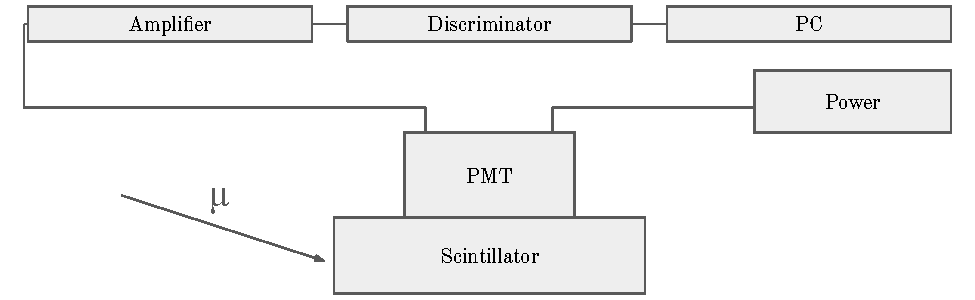
\includegraphics{setup.pdf}
	\caption{\label{fig:setup}The experimental apparatus. The apparatus consists of a scintallator that is amplified by a photomultiplier tube. The signal is then processed through an amplifier and discriminator and is recorded as a detected muon.}
\end{figure*}
Figure \ref{fig:setup} shows the apparatus that was used in this experiment. A scintillator was used to observe muons. When a muon passed through the scintillator it produced a flash of light that was then amplified using a photomultiplier tube. The photomultiplier then triggered the amplifier, creating a positive-going analog voltage pulse. The discriminator filtered out pulses below the threshold voltage. For this experiment, the DC voltage output of the discriminator, a value proportional to the threshold voltage, was set to 200 mV, as per the manufacturer's suggestion. The discriminated pulse was then recorded as a detected muon.
\par
Not all recorded muons give information about muon decay. In order to record muon decay, a second detection of the muon byproducts must be made shortly after the muon was detected. The length of this decay is then recorded. We recorded muon decays for 48 hours.
\par
We plotted the muon decays into a histogram of how many decays occurred at a variety of decay lengths. We used 1 nanosecond bins. This histogram should represent the disintegration curve of the muon. We then fit equation \ref{eq:dis-curve} to our histogram using the python module curve\_fit from the python library SciPy in order to determine the muon lifetime. The histogram, as well as the model, and its residuals, can be seen in figure \ref{fig:results}.
\section{Results}
Figure \ref{fig:results} shows the histogram of muon decays previously discussed in blue, and the model fit in red. A total of 18886 muon decays were recorded. There is a wide spread of residuals at shorter times. This is likely due to uncertainties in measurement as well as non-muon decays that were counted. This fit produced a value of $2.162\pm \SI{.023}{\micro\second}$ for $\tau$.
\begin{figure*}[t]
	\centering
	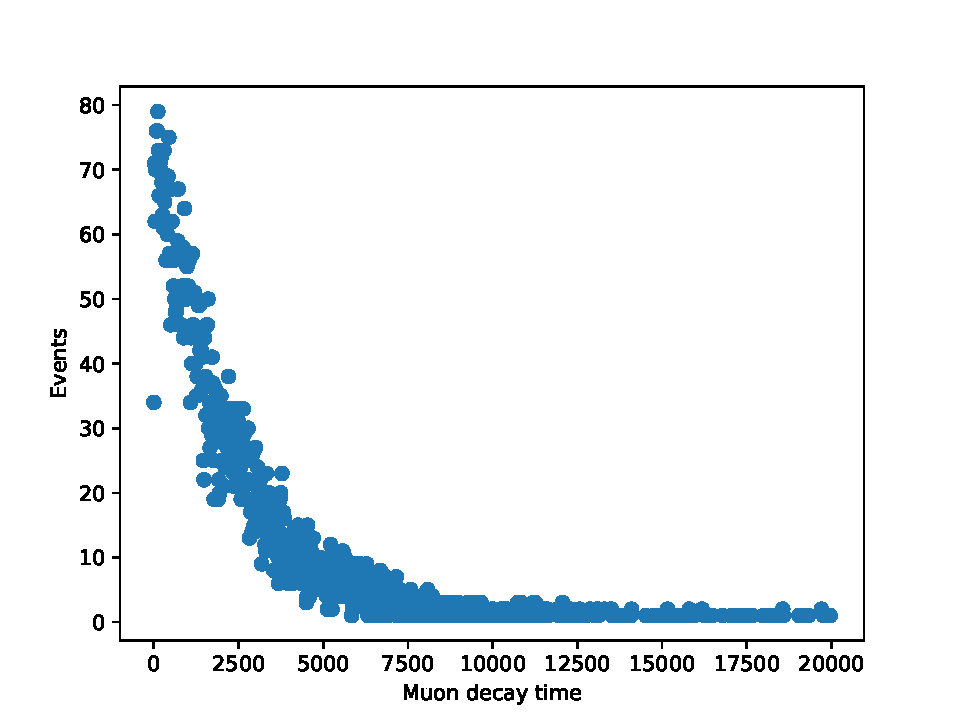
\includegraphics{../python/muon-histogram.pdf}
	\caption{\label{fig:results}The Disintegration Curve and Fitted Model. The upper figure shows how many detected decays were recorded at a variety of decay times in blue, and the modeled disintegration curve in red. The lower figure shows the residual between the model and the data in blue.}
\end{figure*}
Using equation \ref{gf-eq} we can calculate $G_\mathrm{F}/(\hbar c)^3$ (what is known as the reduced Fermi coupling constant) as $\SI{1.18e-5}{}\pm\SI{6.3e-8}{\per\giga\electronvolt\squared}$.
\section{Conclusion}
Our experiment showed, through using a scintallator to detect muons, that the lifetime of a muon is $2.162\pm \SI{.023}{\micro\second}$ for $\tau$. The previously determined value was $2.3\pm \SI{.2}{\micro\second}$ \cite{rossi}. The agreement in values shows that our methods are likely correct. We also used our value of $\tau$ to get a calculated value of the reduced Fermi coupling constant as $\SI{1.18e-5}{}\pm\SI{6.3e-8}{\per\giga\electronvolt\squared}$, this also agrees with previously calculated values.
\par
Understanding the decay time of the muon allows for us to have a deeper understanding of how this lepton exists. Furthermore, with our understanding of the lifetime and the Fermi coupling constant we are able to gain an understanding of the weak interaction and how it interacts with fundamental particles.
\section{Improvement from draft}
I expanded on the conclusion. I reworded the introduction, abstract, results and conclusion to emphasise the importance of the experiment more. I calculated the Fermi coupling constant from the muon lifetime. I added another citation.
\bibliography{sources}
\bibliographystyle{prl}
\end{document}
